\chapter{化学平衡：商与常数}\label{ch:g12:equilibrium}

密封的汽水可数月保持气泡；开盖后，
汽水一下午便失去气泡。两种情况都没有异常。
密闭瓶中，二氧化碳从水中逸出又回到水中，
两者速率相同，组成保持不变；打开瓶盖后，逸出的气体
不再返回。许多反应与之类似：它们在\omterm{def:g7:chemical-reactions:reactant}{反应物}
尚未耗尽时就停止了，处于两个相反反应之间的
平衡。本章用一个数描述这种平衡。

\begin{recall}
\omterm{def:g10:reaction-progress-table:extent}{反应进度} $x$、\omterm{def:g10:reaction-progress-table:limiting}{最大反应进度} $x_{\max}$，以及
达到该值的\omterm{def:g10:reaction-progress-table:limiting}{完全反应}（\cref{ch:g10:reaction-progress-table}）。反应速率与
\omterm{def:g12:reaction-rates:kinetic-factor}{动力学因素}（\cref{ch:g12:reaction-rates}）；\omterm{def:g12:catalysis:catalyst}{催化剂}不改变
\omterm{def:g10:reaction-progress-table:system}{最终状态}（\cref{ch:g12:catalysis}）。
\end{recall}

\begin{omfigure}
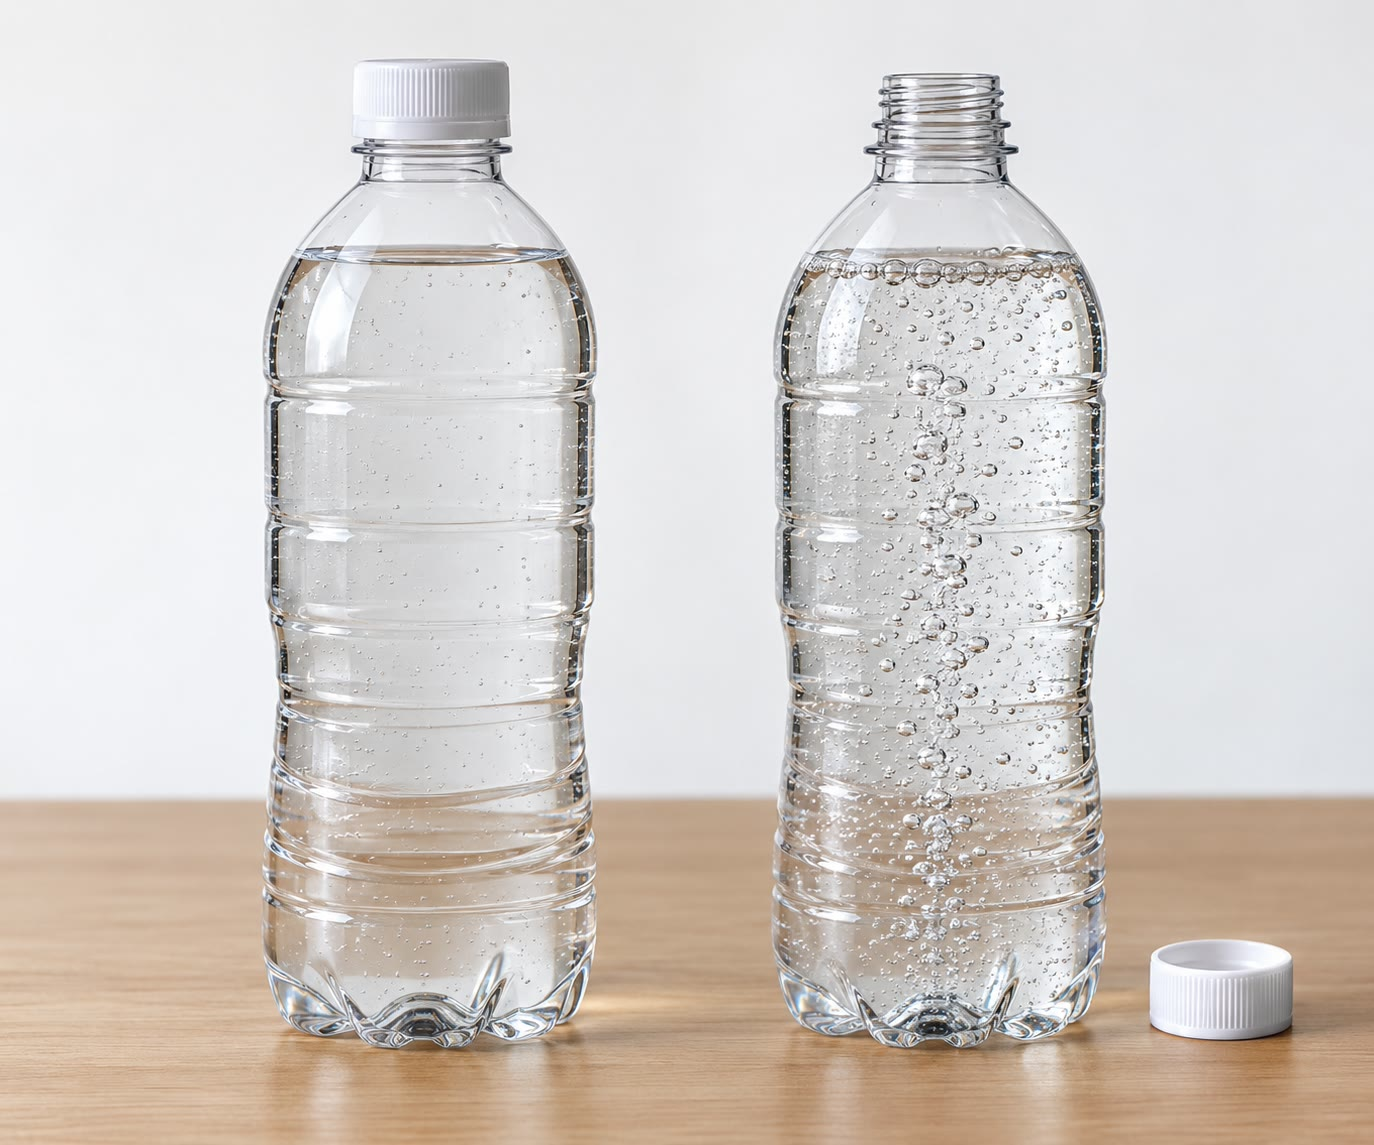
\includegraphics[width=0.45\linewidth,height=5cm,keepaspectratio]{images/book1/ai/g12-fizzy-bottles.jpg}

{\small 密封时，水保持其中的气体；开盖后，气体逸出，
不再返回。}
\end{omfigure}

\section{非完全反应}

\begin{definition}[非完全反应，最终转化率]\label{def:g12:equilibrium:non-total}
若某反应为\emph{非完全反应}\index{非完全反应}，它在
最终\omterm{def:g10:reaction-progress-table:extent}{反应进度} $x_f$ 小于\omterm{def:g10:reaction-progress-table:limiting}{最大反应进度} $x_{\max}$ 时停止，
且所有\omterm{def:g7:chemical-reactions:reactant}{反应物}仍然存在。其\emph{最终
转化率}\index{最终转化率}定义为
\[
  \tau = \frac{x_f}{x_{\max}}, \qquad 0 < \tau < 1
\]
（\omterm{def:g10:reaction-progress-table:limiting}{完全反应}时 $\tau = 1$）。
\end{definition}

\begin{example}[一种中途即停的酯化反应]\label{ex:g12:equilibrium:berthelot}
% ledger: ester:berthelot
将 \qty{1}{mol} 乙醇与 \qty{1}{mol} 乙酸加热，生成
乙酸乙酯和水，
\ce{CH3COOH + C2H5OH <=> CH3COOC2H5 + H2O}。反应约在
三分之二的乙酸参与反应时停止：$x_f = \qty{0.67}{mol}$，
对应 $x_{\max} = \qty{1}{mol}$，故 $\tau \approx 0.67$。从
\qty{1}{mol} 乙酸乙酯和 \qty{1}{mol} 水出发，逆反应
也会停止，约三分之一的酯发生了水解，
两者最终得到相同的\omterm{def:g6:pure-substances-and-mixtures:mixture}{混合物}。
\end{example}

\begin{history}[贝特洛与佩安·德·圣吉尔，1862 年]
% ledger: ester:berthelot
化学家马塞兰·贝特洛与莱昂·佩安·德·圣吉尔曾
将乙酸与乙醇、乙酸乙酯与水的\omterm{def:g6:pure-substances-and-mixtures:mixture}{混合物}
长时间加热，并对其进行分析。由等量的酸与
醇出发，反应总是停在约三分之二处；由酯与
水出发，水解约三分之一即停止。他们还注意到，
各时刻生成酯的量取决于\omterm{def:g7:chemical-reactions:reactant}{反应物}用量的乘积。
他们的工作
是最早的化学平衡定量研究之一。
\end{history}

\section{平衡状态}

\begin{definition}[平衡状态]\label{def:g12:equilibrium:equilibrium-state}
当系统处于\emph{平衡状态}\index{平衡状态}时，
其组成不再改变，尽管正、逆两个反应
仍在进行，且速率相等。能够达到这种状态的反应
用双向箭头 $\rightleftharpoons$ 表示。
\end{definition}

\begin{omfigure}
\begin{tikzpicture}
\begin{axis}[width=0.8\linewidth, height=6cm, xmin=0, xmax=200, ymin=0,
    ymax=1.05, xlabel={$t$ (\si{h})}, ylabel={酯的物质的量 (\si{mol})},
    axis lines*=left, ymajorgrids, grid style={gray!20},
    tick label style={font=\small}, label style={font=\small},
    legend style={font=\small, at={(0.98,0.98)}, anchor=north east,
    draw=none, fill=white}, legend cell align=left]
  % ledger: ester:berthelot (K = 4; kinetics synthetic)
  \addplot[very thick, omDef] table[x=t, y=fromAcid] {figdata/out/grade-12-equilibrium.dat};
  \addplot[very thick, omProp] table[x=t, y=fromEster] {figdata/out/grade-12-equilibrium.dat};
  \addplot[dashed, black!60] coordinates {(0,0.6667) (200,0.6667)};
  \legend{由 1 摩尔酸与 1 摩尔醇出发, 由 1 摩尔酯与 1 摩尔水出发}
  \node[font=\small, anchor=north east] at (axis cs:195,0.65) {平衡：$\tfrac{2}{3}$ 摩尔};
\end{axis}
\end{tikzpicture}

{\small 酯化反应（蓝色）与酯的水解
（橙色）从相反两侧达到相同的平衡组成。
（时间尺度为模型假设，终值为实测值。）}
\end{omfigure}

\section{反应商}

\begin{notation}[标准浓度]\label{not:g12:equilibrium:c-standard}
$c^\circ = \qty{1}{mol/L}$ 为标准浓度。将一个浓度除以
$c^\circ$，所得为一个无单位的数，其数值
与该浓度相同：$[\ce{A}]/c^\circ$。
\end{notation}

\begin{definition}[反应商]\label{def:g12:equilibrium:quotient}
对溶液中的反应 $a\,\ce{A} + b\,\ce{B} \rightleftharpoons c\,\ce{C} + d\,\ce{D}$，系统在某一状态下的\emph{反应
商}\index{反应商}为
\[
  Q = \frac{\left([\ce{C}]/c^\circ\right)^c \left([\ce{D}]/c^\circ\right)^d}
           {\left([\ce{A}]/c^\circ\right)^a \left([\ce{B}]/c^\circ\right)^b} .
\]
固体与\omterm{def:g6:solutions-and-solubility:solute}{溶剂}（\omterm{def:g6:solutions-and-solubility:solute}{水溶液}中为水）不出现在
$Q$ 中。
\end{definition}


\begin{example}[写出反应商]\label{ex:g12:equilibrium:quotients}
在水中发生的 \ce{CH3COOH + H2O <=> CH3COO- + H3O+} 反应（其中\omterm{def:g9:ions:ion}{离子} \ce{H3O+}
将在下一章引入），水为\omterm{def:g6:solutions-and-solubility:solute}{溶剂}：
$Q = \dfrac{[\ce{CH3COO-}]\,[\ce{H3O+}]}{[\ce{CH3COOH}]\,c^\circ}$。对固体的
\omterm{def:g2:mixing-and-dissolving:dissolve}{溶解} \ce{AgCl(s) <=> Ag+ + Cl-}，固体不计入：
$Q = [\ce{Ag+}][\ce{Cl-}]/(c^\circ)^2$。对于酯化反应，四种
物质处于体积为 $V$ 的同一液态\omterm{def:g6:pure-substances-and-mixtures:mixture}{混合物}中，体积
相消，$Q = \dfrac{n_{\text{酯}}\, n_{\text{水}}}{n_{\text{酸}}\, n_{\text{醇}}}$。
\end{example}

\section{平衡常数}

\begin{definition}[平衡常数]\label{def:g12:equilibrium:constant}
\omterm{def:g12:equilibrium:equilibrium-state}{平衡状态}下\omterm{def:g12:equilibrium:quotient}{反应商}的值 $Q_{eq}$ 称为该反应的
\emph{平衡常数}\index{平衡常数} $K$。它没有单位。
它没有单位。
\end{definition}

\begin{proposition}[$K$ 仅取决于温度]\label{prop:g12:equilibrium:constant}
对给定的反应，在给定温度下的任一\omterm{def:g12:equilibrium:equilibrium-state}{平衡状态}中 $Q_{eq} = K$，
与初始\omterm{def:g10:the-mole:amount}{物质的量}无关。
\end{proposition}

\begin{proof}
在本阶段不加证明地承认，其推导见本科二年级分册。以酯化反应为例
进行检验：图中两次实验分别从相反的两侧出发，
所得的 $Q_{eq}$ 相同。
\end{proof}

\begin{example}[酯化反应的 $K$]\label{ex:g12:equilibrium:k-ester}
% ledger: ester:berthelot
取 \qty{1}{mol} 酸与 \qty{1}{mol} 醇，平衡时
含酯和水各 $\frac{2}{3}$ \omterm{def:g10:the-mole:amount}{摩尔}，
酸和醇各 $\frac{1}{3}$ \omterm{def:g10:the-mole:amount}{摩尔}：
\[
  K = \frac{(2/3)\times(2/3)}{(1/3)\times(1/3)} = 4 .
\]
\end{example}

\begin{method}[非完全反应的最终状态]\label{met:g12:equilibrium:final}
\begin{enumerate}
  \item 以未知的最终\omterm{def:g10:reaction-progress-table:extent}{反应进度} $x_f$ 填写\omterm{def:g10:reaction-progress-table:extent}{进度表}。
  \item 将 $Q_{eq}$ 写成 $x_f$ 的函数，并令其等于 $K$。
  \item 求解 $x_f$（常为二次方程），保留
        介于 0 与 $x_{\max}$ 之间的根。
  \item 由此求出最终各\omterm{def:g10:the-mole:amount}{物质的量}及 $\tau = x_f/x_{\max}$。
\end{enumerate}
\end{method}

\begin{example}[醇过量]\label{ex:g12:equilibrium:excess}
取 \qty{1}{mol} 酸与 \qty{2}{mol} 醇，
$\dfrac{x^2}{(1-x)(2-x)} = 4$，即 $3x^2 - 12x + 8 = 0$，
其在 0 与 1 之间的根为 $x_f = \qty{0.845}{mol}$。将醇的用量加倍，
以酸计的\omterm{def:g10:synthesis-yield:yield}{产率}由 \qty{67}{\percent} 提高到
\qty{85}{\percent}。
\end{example}

\section{反应方向的预测与移动}

\begin{proposition}[反应的移动方向]\label{prop:g12:equilibrium:direction}
若 $Q < K$，系统向正反应方向进行（生成物
增加），直至 $Q = K$；若 $Q > K$，则向逆反应方向进行；
若 $Q = K$，则处于\omterm{def:g12:equilibrium:equilibrium-state}{平衡状态}，不再变化。
\end{proposition}

\begin{proof}
在本阶段不加证明地承认：正反应进行时 $Q$ 增大（\omterm{def:g7:atoms-and-molecules:molecule}{分子}中的生成物
增大，分母中的\omterm{def:g7:chemical-reactions:reactant}{反应物}减小），系统
趋向于 $Q = K$ 的状态。
\end{proof}

\begin{omfigure}
\begin{tikzpicture}[font=\small]
  \draw[->, thick] (0,0) -- (10,0) node[right] {$Q$};
  \draw[thick] (0,-0.12) -- (0,0.12) node[above] {0};
  \draw[very thick, omThm] (5,-0.25) -- (5,0.25) node[above] {$K$};
  \draw[->, very thick, omDef] (1.2,0.55) -- (4.4,0.55);
  \node[omDef, align=center] at (2.8,1.15) {$Q < K$：正向};
  \draw[->, very thick, omProp] (8.8,0.55) -- (5.6,0.55);
  \node[omProp, align=center] at (7.2,1.15) {$Q > K$：逆向};
  \node[align=center] at (5,-0.75) {$Q = K$：平衡};
\end{tikzpicture}

{\small \omterm{def:g12:equilibrium:quotient}{反应商}总是趋向于该常数。}
\end{omfigure}

\begin{remark}[平衡的移动]\label{rem:g12:equilibrium:shift}
对于\omterm{def:g12:equilibrium:non-total}{非完全反应}，若要得到更多生成物，可加入过量的
一种\omterm{def:g7:chemical-reactions:reactant}{反应物}（取其更廉价者），或在生成时移除一种生成物：二者
均使 $Q < K$ 重新成立，系统向正向移动。移除酯化反应中的水
（可用干燥剂，或将其\omterm{def:g10:chemical-species:distillation}{蒸馏}除去），可
使反应几乎完全进行。打开的汽水瓶
中逸出的二氧化碳起到同样的作用。
\end{remark}

\begin{omfigure}
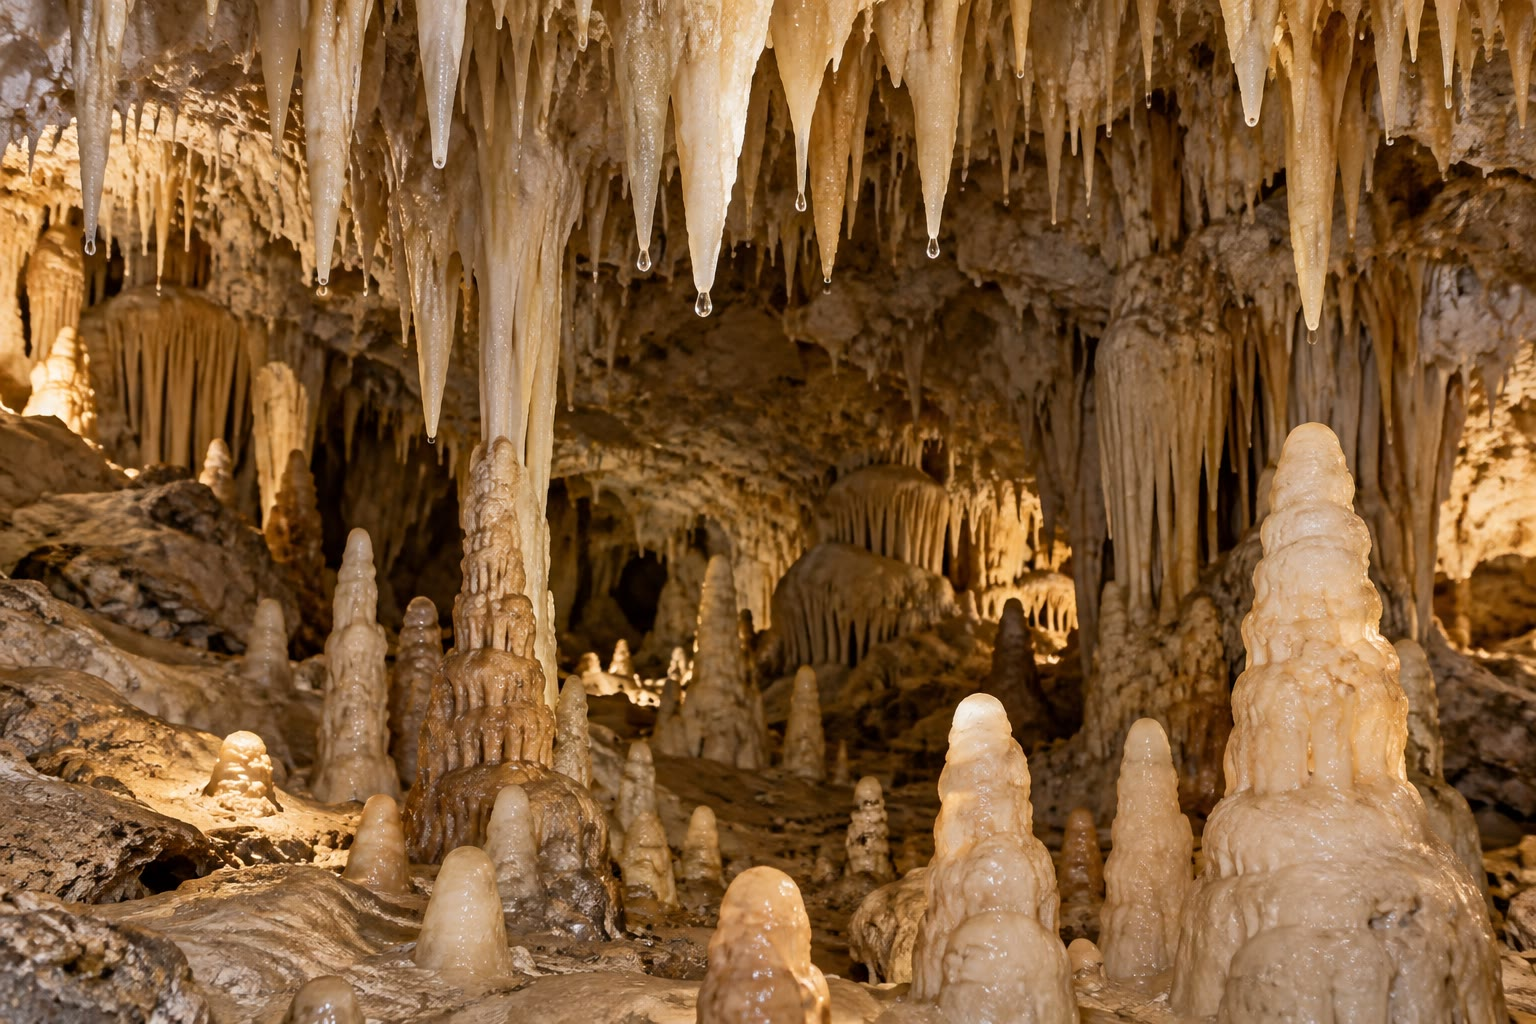
\includegraphics[width=0.45\linewidth]{images/book1/ai/g12-cave-stalactites.jpg}

{\small 钟乳石生长于洞穴中滴水
向\omterm{def:g4:air-a-mixture-of-gases:air}{空气}释放二氧化碳的地方：\omterm{def:g2:mixing-and-dissolving:dissolve}{溶解}的石灰岩平衡发生移动，
使碳酸钙沉积下来。}
\end{omfigure}

\section{练习}

\begin{exercise}[$\star$]\label{exo:g12:equilibrium:1}
写出下列反应的\omterm{def:g12:equilibrium:quotient}{反应商}：（a）\ce{N2 + 3H2 <=> 2NH3}（气体，用
浓度表示）；（b）\ce{CH3COOH + H2O <=> CH3COO- + H3O+} 在水中；
（c）\ce{CaCO3(s) <=> Ca^{2+} + CO3^{2-}}；（d）\ce{Fe^{3+} + SCN- <=>
FeSCN^{2+}}。
\end{exercise}

\begin{exercise}[$\star$]\label{exo:g12:equilibrium:2}
某反应的 $x_{\max} = \qty{0.050}{mol}$，并达到
$x_f = \qty{0.020}{mol}$。计算 $\tau$。该反应是否为\omterm{def:g10:reaction-progress-table:limiting}{完全反应}？
\end{exercise}

\begin{exercise}[$\star$]\label{exo:g12:equilibrium:3}
对于 $K = 10$ 的反应，\omterm{def:g6:pure-substances-and-mixtures:mixture}{混合物}在下列情况下将向哪个方向演变：
$Q = 2$ 时？$Q = 50$ 时？$Q = 10$ 时？
\end{exercise}

\begin{exercise}[$\star$]\label{exo:g12:equilibrium:4}
试说明为什么称平衡是“动态的”。
\end{exercise}

\begin{exercise}[$\star$]\label{exo:g12:equilibrium:5}
\omterm{def:g12:catalysis:catalyst}{催化剂}会改变 $K$ 吗？会改变达到平衡所需的时间吗？请说明理由。
\end{exercise}

\begin{exercise}[$\star\star$]\label{exo:g12:equilibrium:6}
将 \qty{2.0}{mol} 乙酸与 \qty{2.0}{mol} 乙醇\omterm{def:g2:mixing-and-dissolving:mix}{混合}，
（$K = 4$）。计算四种物质的最终\omterm{def:g10:the-mole:amount}{物质的量}。
\end{exercise}

\begin{exercise}[$\star\star$]\label{exo:g12:equilibrium:7}
某\omterm{def:g6:pure-substances-and-mixtures:mixture}{混合物}中乙酸、乙醇、乙酸乙酯和水各
含 \qty{0.5}{mol}。计算 $Q$，该\omterm{def:g6:pure-substances-and-mixtures:mixture}{混合物}将向哪个方向演变？
\end{exercise}

\begin{exercise}[$\star\star$]\label{exo:g12:equilibrium:8}
根据两次实验的图像，读出
各次实验中 \qty{20}{h} 后酯的\omterm{def:g10:the-mole:amount}{物质的量}。体系何时可视为
处于\omterm{def:g12:equilibrium:equilibrium-state}{平衡状态}？
\end{exercise}

\begin{exercise}[$\star\star$]\label{exo:g12:equilibrium:9}
从 \qty{1}{mol} 酯和 \qty{1}{mol} 水出发（酯化反应的 $K = 4$，
故水解反应的\omterm{def:g12:equilibrium:constant}{平衡常数}为 $1/4$），用本章的方法计算
最终\omterm{def:g10:the-mole:amount}{物质的量}，并与酯化
实验进行比较。
\end{exercise}

\begin{exercise}[$\star\star$]\label{exo:g12:equilibrium:10}
为什么固体不出现在
\ce{AgCl(s) <=> Ag+ + Cl-} 的\omterm{def:g12:equilibrium:quotient}{反应商}中？加入更多固体是否会使
平衡发生移动？
\end{exercise}

\begin{exercise}[$\star\star$]\label{exo:g12:equilibrium:11}
在密闭的一瓶汽水中，二氧化碳逸出和溶入
水中的速率相同。写出平衡
\ce{CO2(aq) <=> CO2(g)}，并结合 $Q$ 和 $K$ 说明，打开瓶盖后汽水为何
会失去气泡。
\end{exercise}

\begin{exercise}[$\star\star\star$]\label{exo:g12:equilibrium:12}
用 \qty{1}{mol} 酸与 \qty{1}{mol} 醇进行酯化反应，
达到平衡后，移去一半的水。计算
新的 $Q$，说明体系将向哪个方向演变，并求
新平衡时酯的最终\omterm{def:g10:the-mole:amount}{物质的量}。
\end{exercise}

\begin{exercise}[$\star\star\star$]\label{exo:g12:equilibrium:13}
证明逆反应的\omterm{def:g12:equilibrium:constant}{平衡常数}为 $1/K$。
乙酸乙酯水解反应的\omterm{def:g12:equilibrium:constant}{平衡常数}是多少？
\end{exercise}

\begin{exercise}[$\star\star\star$]\label{exo:g12:equilibrium:14}
某化学家将 \qty{1}{mol} 酸、\qty{1}{mol} 醇、
\qty{2}{mol} 酯和 \qty{0.5}{mol} 水\omterm{def:g2:mixing-and-dissolving:mix}{混合}。会发生反应吗？
请说明理由。
\end{exercise}

\begin{exercise}[$\star\star\star$]\label{exo:g12:equilibrium:15}
需要过量多少醇（以每\omterm{def:g10:the-mole:amount}{摩尔}酸计的\omterm{def:g10:the-mole:amount}{物质的量}），
才能使 \qty{95}{\percent} 的酸发生酯化？解方程 $\dfrac{0.95^2}{0.05(n - 0.95)} =
4$。
\end{exercise}

\section{问题：贝特洛的酯}

\begin{problem}[{周末问题——当醇以
三倍过量加入时，能得到多少酯？}]
\label{pb:g12:equilibrium:1}
% ledger: ester:berthelot, aw:C, aw:H, aw:O
乙酸乙酯是一种\omterm{def:g6:solutions-and-solubility:solute}{溶剂}和香料，由乙酸
与乙醇制得。1862 年，贝特洛与佩安·德·圣吉尔
发现，取等量的酸和醇时，反应
进行到约三分之二的酸发生反应时即停止。

\medskip
\noindent\textbf{第一部分——反应。}
\begin{enumerate}
  \item 写出酯化反应的方程式，
        并用\omterm{def:g11:organic-skeletons:formulas}{结构简式}表示。
  \item 为什么用双箭头表示？
  \item 用\omterm{def:g10:the-mole:amount}{物质的量}写出其\omterm{def:g12:equilibrium:quotient}{反应商}。
  \item 从 \qty{1}{mol} 酸和 \qty{1}{mol} 醇出发，
        $x_{\max}$ 为多少？根据贝特洛的结果，$x_f$ 为多少？
  \item 计算 $\tau$。
\end{enumerate}

\medskip
\noindent\textbf{第二部分——\omterm{def:g12:equilibrium:constant}{平衡常数}。}
\begin{enumerate}[resume]
  \item 给出四种物质的最终\omterm{def:g10:the-mole:amount}{物质的量}。
  \item 计算 $K$。
  \item 从 \qty{1}{mol} 酯和 \qty{1}{mol} 水出发，
        贝特洛发现有三分之一发生了水解。证明该结果与
        同一 $K$ 值相符。
  \item 为什么两种情况下 $K$ 必须相同？
\end{enumerate}

\medskip
\noindent\textbf{第三部分——醇的三倍过量。}
\begin{enumerate}[resume]
  \item 从 \qty{1}{mol} 酸和 \qty{3}{mol} 醇出发，填写
        \omterm{def:g10:reaction-progress-table:extent}{进度表}。
  \item 写出方程 $Q_{eq} = K$，并证明它可化为
        $3x^2 - 16x + 12 = 0$。
  \item 解此方程，并取有意义的根。
  \item 酸的多大比例发生了酯化？
  \item 计算所得酯的质量。
\end{enumerate}

\medskip
\noindent\textbf{第四部分——移去水。}
\begin{enumerate}[resume]
  \item 从等\omterm{def:g10:the-mole:amount}{物质的量}的平衡出发，生成的水随即
        被移去。用 $Q$ 说明反应为何仍会继续进行。
  \item 若水能全部移去，\omterm{def:g10:synthesis-yield:yield}{产率}将变为多少？
  \item 为什么通常过量的是醇而不是酸？（想一想
        成本以及如何分离产物。）
  \item 加热\omterm{def:g6:pure-substances-and-mixtures:mixture}{混合物}会改变\omterm{def:g10:reaction-progress-table:system}{最终状态}，还是只改变
        达到该状态所需的时间？（酯化反应几乎不放热。）
  \item 给出最终答案：在醇过量三倍时，酸的多大比例
        发生了酯化？
\end{enumerate}
\end{problem}
